%%%%%%%%%%%%%%%%%%%%%%%%%%%%%%%%%%%%%%%%%
% FRI Data Science_report LaTeX Template
% Version 1.0 (28/1/2020)
%
% Jure Demšar (jure.demsar@fri.uni-lj.si)
%
% Based on MicromouseSymp article template by:
% Mathias Legrand (legrand.mathias@gmail.com)
% With extensive modifications by:
% Antonio Valente (antonio.luis.valente@gmail.com)
%
% License:
% CC BY-NC-SA 3.0 (http://creativecommons.org/licenses/by-nc-sa/3.0/)
%
%%%%%%%%%%%%%%%%%%%%%%%%%%%%%%%%%%%%%%%%%


%----------------------------------------------------------------------------------------
%	PACKAGES AND OTHER DOCUMENT CONFIGURATIONS
%----------------------------------------------------------------------------------------
\documentclass[fleqn,moreauthors,10pt]{ds_report}
\usepackage[english]{babel}

\graphicspath{{fig/}}




%----------------------------------------------------------------------------------------
%	ARTICLE INFORMATION
%----------------------------------------------------------------------------------------

% Header
\JournalInfo{Machine Learning for Data Science 1, 2025-2026}

% Interim or final report
%\Archive{Interim report}
\Archive{Homework 1 Report}

% Article title
\PaperTitle{Classification Trees, Random Forests}

% Authors and their info
\Authors{Tjaš Ajdovec}
\affiliation{\textit{ta5946@fri.uni-lj.si}}

% Multiple authors
%\Authors{John Doe\textsuperscript{1}, Jane Doe\textsuperscript{2}, and Mike Smith\textsuperscript{3}}
%\affiliation{\textsuperscript{1}\textit{john.doe@fri.uni-lj.si}}
%\affiliation{\textsuperscript{1}\textit{jane.doe@fri.uni-lj.si}}
%\affiliation{\textsuperscript{1}\textit{mike.smith@fri.uni-lj.si}}

%----------------------------------------------------------------------------------------

\makeatletter
\renewcommand{\@maketitle}{%
\twocolumn[{%
\thispagestyle{empty}%
{
\includegraphics[height=2cm]{logo}}
\vskip-74pt%
{\raggedleft\small\sffamily\bfseries\@JournalInfo\\\@Archive\par}%
\vskip64pt%
{\raggedright\color{color1}\fontfamily{cmss}\fontseries{bc}\fontshape{n}\fontsize{20}{25}\selectfont \@PaperTitle\par}%
\vskip10pt%
{\raggedright\color{color1}\sffamily\fontsize{12}{16}\selectfont  \@Authors\par}%
\vskip8pt%
\begingroup%
\raggedright\sffamily\small%
\footnotesize\@affiliation\par%
\endgroup%
\vskip10pt%
}]%
}
\makeatother

\begin{document}

% Makes all text pages the same height
\flushbottom

% Print the title and abstract box
\maketitle

% Removes page numbering from the first page
\thispagestyle{empty}

%----------------------------------------------------------------------------------------
%	ARTICLE CONTENTS
%----------------------------------------------------------------------------------------

\section*{Introduction}
    In this homework we implemented \textbf{classification trees and random forests} (RFs). We used a dataset of high dimensional spectral data labeled with 2 genetic states. We evaluated full classification trees and random forests with bootstrap sampling. We also compared the results, estimated uncertainty and feature importance. 

%------------------------------------------------

\section*{Methods}

Binary classification trees search over all features and value midpoints to select the split that minimizes data impurity at each training step. This is measured with a \textbf{weighted Gini index} ($k=2$):

\begin{equation}
G_{\text{weighted}} = \sum_{i=1}^{k} \frac{n_i}{n} \left(1 - \sum_{j=1}^{C} p_{ij}^2 \right)
\end{equation}

The trees are built recursively until the node is pure or contains less than the predetermined minimum number of samples. Random forests decorrelate trees in two ways. Each tree considers only $\sqrt{m}$ features for a split and is built on a bootstrap data sample. Because this is a binary classification task we quantified uncertainty with \textbf{Bernoulli proportion standard error}:

\begin{equation}
SE_{Bern} = \sqrt{\frac{p (1 - p)}{n}}
\end{equation}

Where $p$ is the observed error rate and $n$ is the test set size. We estimated feature importance of a random forests as the average of its 100 trees. We calculated the feature importance for each RF tree by \textbf{measuring the accuracy drop on its out-of-bag (OOB) samples} after permuting the feature values. We normalized the RF feature importance and compared it with root split frequency on a dataset with randomly shuffled labels to account for inherent feature characteristics, such as variance.

%------------------------------------------------

\section*{Results}

First we trained the classification models on a set of 128 instances and tested them on 60 instances. The class labels were either a mutated "Bcr-abl" or normal "Wild type" state. The misclassification rates are presented in Table \ref{tab1}. We observed that both models perfectly fit the training data, while the \textbf{RF had a 4\% higher classification accuracy} (lower error) on the test set.

\begin{table}[h!]
    \centering
    \begin{tabular}{lcc}
        \toprule
        \textbf{Model} & \textbf{Train error} & \textbf{Test error} \\
        \midrule
        Full Tree       & $0.00 \pm 0.00$ & $\textbf{0.27} \pm 0.06$ \\
        Random Forest   & $0.00 \pm 0.00$ & $\textbf{0.23} \pm 0.05$ \\
        \bottomrule
    \end{tabular}
    \vspace{0.5em}
    \caption{Train and test set misclassification rate and standard error for a full tree and random forest with a 100 trees.}
    \label{tab1}
\end{table}

Secondly, we evaluated RFs with different number of trees. The misclassification rates and standard errors (shaded area) for both the train and test set are plotted on Figure \ref{fig1}. We observed that the \textbf{training error converges to 0 after around 30 trees}. The \textbf{testing error stabilizes but moves between 0.20 and 0.25}, which is likely a consequence of random feature selection in high-dimensional data.

Lastly, we quantified the RF feature importance and compared them to relative root split frequency on a randomized training dataset. Figure \ref{fig2} shows higher importance of \textbf{features in spectral regions 260-300 and 340-400} (in blue). This only partially overlaps with their root split frequency.

\begin{figure*}[htb]
    \centering
	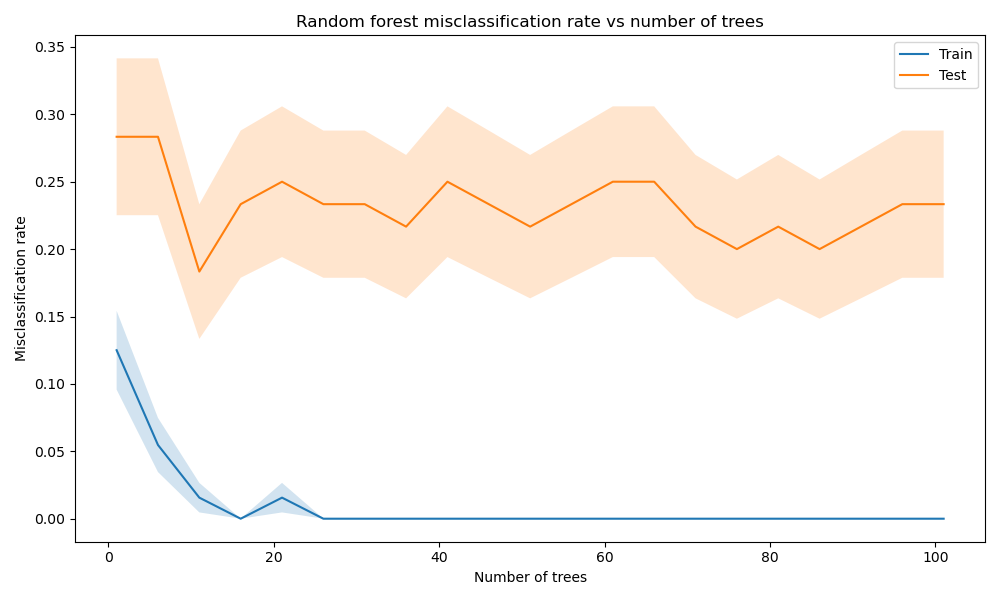
\includegraphics[width=0.8\textwidth]{fig/rf_misclassification.png}
	\caption{Random forest misclassification rate for increasing number of trees.}
	\label{fig1}
\end{figure*}

\begin{figure*}[htb]
    \centering
    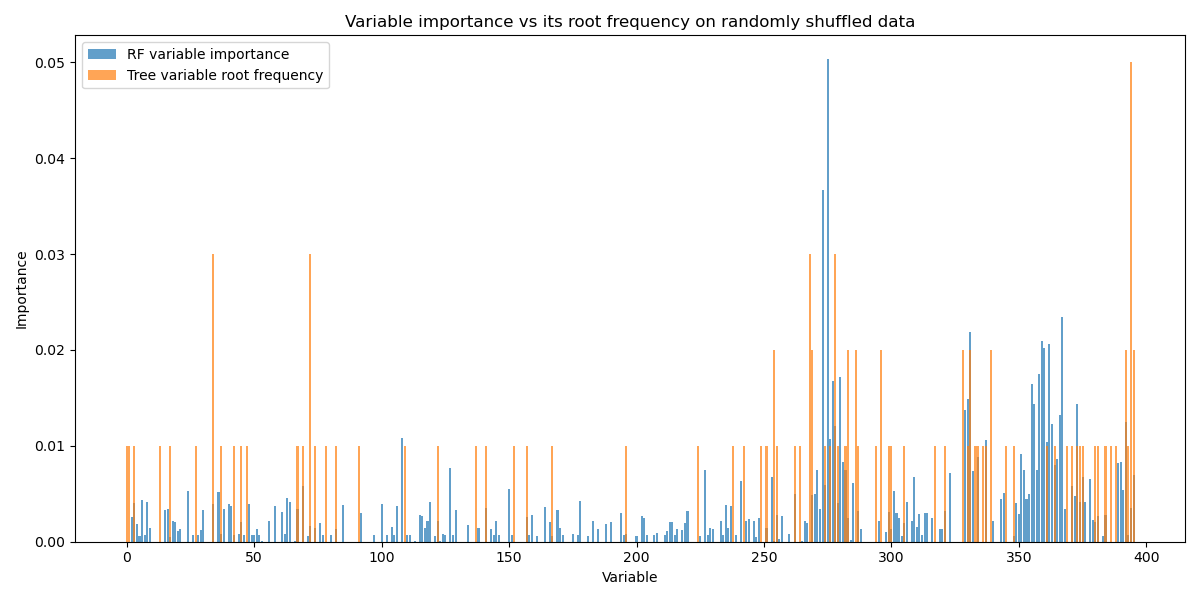
\includegraphics[width=\textwidth]{fig/variable_importance.png}
    \caption{Random forest permutation feature importance.}
    \label{fig2}
\end{figure*}

%------------------------------------------------

\section*{Discussion}

We concluded that random forests offer a noticeable performance gain over full trees while still having relatively simple feature importance algorithms. Due to a very limited dataset the test set misclassification rate stayed at 23\%. This could be improved with more training data or a \textbf{more sophisticated tree building approach}.

\end{document}
